% Density-Based Spatial Clustering of Applications with Noise
\begin{frame}[allowframebreaks]{Clustering - Density-Based Methods}
\begin{itemize}
    \setlength{\itemsep}{0.1em}
    \item Clustering based on density (local cluster criterion), such as density-connected points or based on an explicitly constructed density function.
    \item \textbf{Major features}:
    \begin{itemize}
        \item Discover clusters of arbitrary shape
        \item Handle noise
        \item One scan
        \item Need density parameters
    \end{itemize}

    \framebreak
    
    \item \textbf{Major algorithms}:
    \begin{itemize}
        \item DBSCAN (Density-Based Spatial Clustering of Applications with Noise): Ester, et al. (KDD’96)
        \item OPTICS (Ordering Points to Identify the Clustering Structure): Ankerst, et al. (SIGMOD’99)
        \item HDBSCAN (Hierarchical Density-Based Spatial Clustering of Applications with Noise): Campello, et al. (ACM TIST’15)
        \item DENCLUE (DENsity-based CLUstEring): Hinneburg and Gabriel (KDD’97)
        \item CLIQUE (CLustering In QUEst): Karypis, Han, and Kumar (SIGMOD’98)
    \end{itemize}
\end{itemize}
\end{frame}

\begin{frame}[allowframebreaks]{Clustering - DBSCAN}
\begin{itemize}
    \item \textbf{DBSCAN} (Density-Based Spatial Clustering of Applications with Noise):
    \begin{itemize}
        \item Density = number of points within a specified radius $\epsilon$.
        \item A point is a core point if it has more than a specified number of points (MinPts) within $\epsilon$. These are points that are at the interior of a cluster.
        \item A border point has fewer than MinPts within $\epsilon$, but is in the neighborhood of a core point
        \item A noise point is any point that is not a core point or a border point.
        \item Groups together points that are closely packed together, marking as outliers points that lie alone in low-density regions.
        \item Parameters:
        \begin{itemize}
            \item $\epsilon$: Maximum distance between two points for them to be considered as in the same neighborhood.
            \item MinPts: Minimum number of points required to form a dense region.
        \end{itemize}
    \end{itemize}
\end{itemize}

\framebreak

\begin{figure}
    \centering
    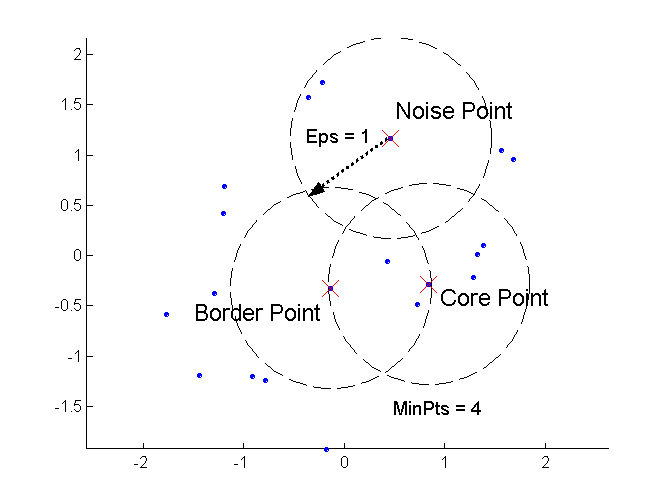
\includegraphics[width=0.95\textwidth,height=0.8\textheight,keepaspectratio]{images/dul/dbscan/dbscan-features.png}
    \caption{DBSCAN features: Core, Border, and Noise Points}
\end{figure}
\end{frame}


\begin{frame}[allowframebreaks]{Clustering - DBSCAN: Algorithm}
\begin{algorithm}[H]
\caption{Graph-Based DBSCAN Clustering}
\KwIn{Set of points $P$, distance threshold $\varepsilon$, minimum number of points $minPts$}
\KwOut{A set of clusters}

Construct a directed graph $G = (V, E)$ where each node in $V$ corresponds to a point in $P$\;

\ForEach{point $c \in P$}{
    \If{$c$ is a core point (i.e., $|\mathcal{N}_\varepsilon(c)| \geq minPts$)}{
        \ForEach{point $p \in \mathcal{N}_\varepsilon(c)$}{
            Add a directed edge $(c \rightarrow p)$ to $E$\;
        }
    }
}

$N \leftarrow V$\;

\While{there exists a core point $c \in N$}{
    Let $X$ be the set of nodes reachable from $c$ via directed edges in $G$\;
    Form a cluster $C = X \cup \{c\}$\;
    Remove all nodes in $C$ from $N$\;
}

\end{algorithm}
\end{frame}

\begin{frame}[allowframebreaks]{Clustering - DBSCAN: Core, Border, and Noise Points}